\documentclass[1p]{elsarticle_modified}
%\bibliographystyle{elsarticle-num}

%\usepackage[colorlinks]{hyperref}
%\usepackage{abbrmath_seonhwa} %\Abb, \Ascr, \Acal ,\Abf, \Afrak
\usepackage{amsfonts}
\usepackage{amssymb}
\usepackage{amsmath}
\usepackage{amsthm}
\usepackage{scalefnt}
\usepackage{amsbsy}
\usepackage{kotex}
\usepackage{caption}
\usepackage{subfig}
\usepackage{color}
\usepackage{graphicx}
\usepackage{xcolor} %% white, black, red, green, blue, cyan, magenta, yellow
\usepackage{float}
\usepackage{setspace}
\usepackage{hyperref}

\usepackage{tikz}
\usetikzlibrary{arrows}

\usepackage{multirow}
\usepackage{array} % fixed length table
\usepackage{hhline}

%%%%%%%%%%%%%%%%%%%%%
\makeatletter
\renewcommand*\env@matrix[1][\arraystretch]{%
	\edef\arraystretch{#1}%
	\hskip -\arraycolsep
	\let\@ifnextchar\new@ifnextchar
	\array{*\c@MaxMatrixCols c}}
\makeatother %https://tex.stackexchange.com/questions/14071/how-can-i-increase-the-line-spacing-in-a-matrix
%%%%%%%%%%%%%%%

\usepackage[normalem]{ulem}

\newcommand{\msout}[1]{\ifmmode\text{\sout{\ensuremath{#1}}}\else\sout{#1}\fi}
%SOURCE: \msout is \stkout macro in https://tex.stackexchange.com/questions/20609/strikeout-in-math-mode

\newcommand{\cancel}[1]{
	\ifmmode
	{\color{red}\msout{#1}}
	\else
	{\color{red}\sout{#1}}
	\fi
}

\newcommand{\add}[1]{
	{\color{blue}\uwave{#1}}
}

\newcommand{\replace}[2]{
	\ifmmode
	{\color{red}\msout{#1}}{\color{blue}\uwave{#2}}
	\else
	{\color{red}\sout{#1}}{\color{blue}\uwave{#2}}
	\fi
}

\newcommand{\Sol}{\mathcal{S}} %segment
\newcommand{\D}{D} %diagram
\newcommand{\A}{\mathcal{A}} %arc


%%%%%%%%%%%%%%%%%%%%%%%%%%%%%5 test

\def\sl{\operatorname{\textup{SL}}(2,\Cbb)}
\def\psl{\operatorname{\textup{PSL}}(2,\Cbb)}
\def\quan{\mkern 1mu \triangleright \mkern 1mu}

\theoremstyle{definition}
\newtheorem{thm}{Theorem}[section]
\newtheorem{prop}[thm]{Proposition}
\newtheorem{lem}[thm]{Lemma}
\newtheorem{ques}[thm]{Question}
\newtheorem{cor}[thm]{Corollary}
\newtheorem{defn}[thm]{Definition}
\newtheorem{exam}[thm]{Example}
\newtheorem{rmk}[thm]{Remark}
\newtheorem{alg}[thm]{Algorithm}

\newcommand{\I}{\sqrt{-1}}
\begin{document}

%\begin{frontmatter}
%
%\title{Boundary parabolic representations of knots up to 8 crossings}
%
%%% Group authors per affiliation:
%\author{Yunhi Cho} 
%\address{Department of Mathematics, University of Seoul, Seoul, Korea}
%\ead{yhcho@uos.ac.kr}
%
%
%\author{Seonhwa Kim} %\fnref{s_kim}}
%\address{Center for Geometry and Physics, Institute for Basic Science, Pohang, 37673, Korea}
%\ead{ryeona17@ibs.re.kr}
%
%\author{Hyuk Kim}
%\address{Department of Mathematical Sciences, Seoul National University, Seoul 08826, Korea}
%\ead{hyukkim@snu.ac.kr}
%
%\author{Seokbeom Yoon}
%\address{Department of Mathematical Sciences, Seoul National University, Seoul, 08826,  Korea}
%\ead{sbyoon15@snu.ac.kr}
%
%\begin{abstract}
%We find all boundary parabolic representation of knots up to 8 crossings.
%
%\end{abstract}
%\begin{keyword}
%    \MSC[2010] 57M25 
%\end{keyword}
%
%\end{frontmatter}

%\linenumbers
%\tableofcontents
%
\newcommand\colored[1]{\textcolor{white}{\rule[-0.35ex]{0.8em}{1.4ex}}\kern-0.8em\color{red} #1}%
%\newcommand\colored[1]{\textcolor{white}{ #1}\kern-2.17ex	\textcolor{white}{ #1}\kern-1.81ex	\textcolor{white}{ #1}\kern-2.15ex\color{red}#1	}

{\Large $\underline{12a_{0498}~(K12a_{0498})}$}

\setlength{\tabcolsep}{10pt}
\renewcommand{\arraystretch}{1.6}
\vspace{1cm}\begin{tabular}{m{100pt}>{\centering\arraybackslash}m{274pt}}
\multirow{5}{120pt}{
	\centering
	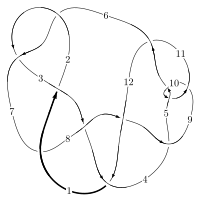
\includegraphics[width=112pt]{../../../GIT/diagram.site/Diagrams/png/1299_12a_0498.png}\\
\ \ \ A knot diagram\footnotemark}&
\allowdisplaybreaks
\textbf{Linearized knot diagam} \\
\cline{2-2}
 &
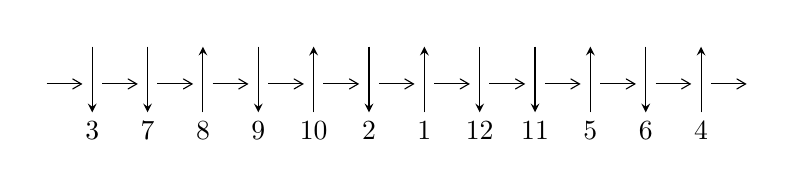
\begin{tikzpicture}[x=20pt, y=17pt]
	% nodes
	\node (C0) at (0, 0) {};
	\node (C1) at (1, 0) {};
	\node (C1U) at (1, +1) {};
	\node (C1D) at (1, -1) {3};

	\node (C2) at (2, 0) {};
	\node (C2U) at (2, +1) {};
	\node (C2D) at (2, -1) {7};

	\node (C3) at (3, 0) {};
	\node (C3U) at (3, +1) {};
	\node (C3D) at (3, -1) {8};

	\node (C4) at (4, 0) {};
	\node (C4U) at (4, +1) {};
	\node (C4D) at (4, -1) {9};

	\node (C5) at (5, 0) {};
	\node (C5U) at (5, +1) {};
	\node (C5D) at (5, -1) {10};

	\node (C6) at (6, 0) {};
	\node (C6U) at (6, +1) {};
	\node (C6D) at (6, -1) {2};

	\node (C7) at (7, 0) {};
	\node (C7U) at (7, +1) {};
	\node (C7D) at (7, -1) {1};

	\node (C8) at (8, 0) {};
	\node (C8U) at (8, +1) {};
	\node (C8D) at (8, -1) {12};

	\node (C9) at (9, 0) {};
	\node (C9U) at (9, +1) {};
	\node (C9D) at (9, -1) {11};

	\node (C10) at (10, 0) {};
	\node (C10U) at (10, +1) {};
	\node (C10D) at (10, -1) {5};

	\node (C11) at (11, 0) {};
	\node (C11U) at (11, +1) {};
	\node (C11D) at (11, -1) {6};

	\node (C12) at (12, 0) {};
	\node (C12U) at (12, +1) {};
	\node (C12D) at (12, -1) {4};
	\node (C13) at (13, 0) {};

	% arrows
	\draw[->,>={angle 60}]
	(C0) edge (C1) (C1) edge (C2) (C2) edge (C3) (C3) edge (C4) (C4) edge (C5) (C5) edge (C6) (C6) edge (C7) (C7) edge (C8) (C8) edge (C9) (C9) edge (C10) (C10) edge (C11) (C11) edge (C12) (C12) edge (C13) ;	\draw[->,>=stealth]
	(C1U) edge (C1D) (C2U) edge (C2D) (C3D) edge (C3U) (C4U) edge (C4D) (C5D) edge (C5U) (C6U) edge (C6D) (C7D) edge (C7U) (C8U) edge (C8D) (C9U) edge (C9D) (C10D) edge (C10U) (C11U) edge (C11D) (C12D) edge (C12U) ;
	\end{tikzpicture} \\
\hhline{~~} \\& 
\textbf{Solving Sequence} \\ \cline{2-2} 
 &
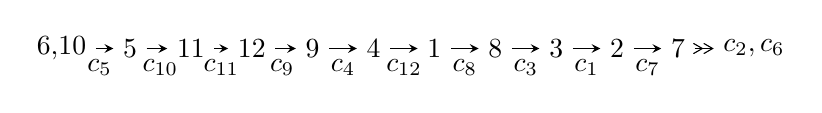
\begin{tikzpicture}[x=22pt, y=7pt]
	% node
	\node (A0) at (-1/8, 0) {6,10};
	\node (A1) at (1, 0) {5};
	\node (A2) at (2, 0) {11};
	\node (A3) at (3, 0) {12};
	\node (A4) at (4, 0) {9};
	\node (A5) at (5, 0) {4};
	\node (A6) at (6, 0) {1};
	\node (A7) at (7, 0) {8};
	\node (A8) at (8, 0) {3};
	\node (A9) at (9, 0) {2};
	\node (A10) at (10, 0) {7};
	\node (C1) at (1/2, -1) {$c_{5}$};
	\node (C2) at (3/2, -1) {$c_{10}$};
	\node (C3) at (5/2, -1) {$c_{11}$};
	\node (C4) at (7/2, -1) {$c_{9}$};
	\node (C5) at (9/2, -1) {$c_{4}$};
	\node (C6) at (11/2, -1) {$c_{12}$};
	\node (C7) at (13/2, -1) {$c_{8}$};
	\node (C8) at (15/2, -1) {$c_{3}$};
	\node (C9) at (17/2, -1) {$c_{1}$};
	\node (C10) at (19/2, -1) {$c_{7}$};
	\node (A11) at (45/4, 0) {$c_{2},c_{6}$};

	% edge
	\draw[->,>=stealth]	
	(A0) edge (A1) (A1) edge (A2) (A2) edge (A3) (A3) edge (A4) (A4) edge (A5) (A5) edge (A6) (A6) edge (A7) (A7) edge (A8) (A8) edge (A9) (A9) edge (A10) ;
	\draw[->>,>={angle 60}]	
	(A10) edge (A11);
\end{tikzpicture} \\ 

\end{tabular} \\

\footnotetext{
The image of knot diagram is generated by the software ``\textbf{Draw programme}" developed by Andrew Bartholomew(\url{http://www.layer8.co.uk/maths/draw/index.htm\#Running-draw}), where we modified some parts for our purpose(\url{https://github.com/CATsTAILs/LinksPainter}).
}\phantom \\ \newline 
\centering \textbf{Ideals for irreducible components\footnotemark of $X_{\text{par}}$} 
 
\begin{align*}
I^u_{1}&=\langle 
u^{103}- u^{102}+\cdots+2 u-1\rangle \\
\\
\end{align*}
\raggedright * 1 irreducible components of $\dim_{\mathbb{C}}=0$, with total 103 representations.\\
\footnotetext{All coefficients of polynomials are rational numbers. But the coefficients are sometimes approximated in decimal forms when there is not enough margin.}
\newpage
\renewcommand{\arraystretch}{1}
\centering \section*{I. $I^u_{1}= \langle u^{103}- u^{102}+\cdots+2 u-1 \rangle$}
\flushleft \textbf{(i) Arc colorings}\\
\begin{tabular}{m{7pt} m{180pt} m{7pt} m{180pt} }
\flushright $a_{6}=$&$\begin{pmatrix}1\\0\end{pmatrix}$ \\
\flushright $a_{10}=$&$\begin{pmatrix}0\\u\end{pmatrix}$ \\
\flushright $a_{5}=$&$\begin{pmatrix}1\\u^2\end{pmatrix}$ \\
\flushright $a_{11}=$&$\begin{pmatrix}u\\u^3+u\end{pmatrix}$ \\
\flushright $a_{12}=$&$\begin{pmatrix}- u^3\\u^3+u\end{pmatrix}$ \\
\flushright $a_{9}=$&$\begin{pmatrix}u^3\\u^5+u^3+u\end{pmatrix}$ \\
\flushright $a_{4}=$&$\begin{pmatrix}- u^6- u^4+1\\- u^8-2 u^6-2 u^4\end{pmatrix}$ \\
\flushright $a_{1}=$&$\begin{pmatrix}u^{17}+4 u^{15}+7 u^{13}+4 u^{11}-3 u^9-6 u^7-2 u^5+u\\u^{19}+5 u^{17}+12 u^{15}+15 u^{13}+9 u^{11}- u^9-4 u^7-2 u^5+u^3+u\end{pmatrix}$ \\
\flushright $a_{8}=$&$\begin{pmatrix}u^{11}+2 u^9+2 u^7+u^3\\- u^{11}-3 u^9-4 u^7- u^5+u^3+u\end{pmatrix}$ \\
\flushright $a_{3}=$&$\begin{pmatrix}u^{30}+7 u^{28}+\cdots-2 u^{12}+1\\- u^{30}-8 u^{28}+\cdots-4 u^6+u^2\end{pmatrix}$ \\
\flushright $a_{2}=$&$\begin{pmatrix}- u^{79}-20 u^{77}+\cdots-20 u^9-8 u^7\\u^{79}+21 u^{77}+\cdots-2 u^5+u\end{pmatrix}$ \\
\flushright $a_{7}=$&$\begin{pmatrix}u^{47}+12 u^{45}+\cdots+20 u^9+8 u^7\\u^{49}+13 u^{47}+\cdots-2 u^5+u\end{pmatrix}$\\&\end{tabular}
\flushleft \textbf{(ii) Obstruction class $= -1$}\\~\\
\flushleft \textbf{(iii) Cusp Shapes $= 4 u^{101}-4 u^{100}+\cdots+8 u-10$}\\~\\
\newpage\renewcommand{\arraystretch}{1}
\flushleft \textbf{(iv) u-Polynomials at the component}\newline \\
\begin{tabular}{m{50pt}|m{274pt}}
Crossings & \hspace{64pt}u-Polynomials at each crossing \\
\hline $$\begin{aligned}c_{1}\end{aligned}$$&$\begin{aligned}
&u^{103}+49 u^{102}+\cdots+2 u^2+1
\end{aligned}$\\
\hline $$\begin{aligned}c_{2},c_{6}\end{aligned}$$&$\begin{aligned}
&u^{103}- u^{102}+\cdots-2 u^3+1
\end{aligned}$\\
\hline $$\begin{aligned}c_{3}\end{aligned}$$&$\begin{aligned}
&u^{103}+u^{102}+\cdots+1790 u+193
\end{aligned}$\\
\hline $$\begin{aligned}c_{4},c_{11}\end{aligned}$$&$\begin{aligned}
&u^{103}- u^{102}+\cdots-25 u+2
\end{aligned}$\\
\hline $$\begin{aligned}c_{5},c_{10}\end{aligned}$$&$\begin{aligned}
&u^{103}+u^{102}+\cdots+2 u+1
\end{aligned}$\\
\hline $$\begin{aligned}c_{7}\end{aligned}$$&$\begin{aligned}
&u^{103}-3 u^{102}+\cdots-1595 u+264
\end{aligned}$\\
\hline $$\begin{aligned}c_{8}\end{aligned}$$&$\begin{aligned}
&u^{103}-13 u^{102}+\cdots-20 u+1
\end{aligned}$\\
\hline $$\begin{aligned}c_{9}\end{aligned}$$&$\begin{aligned}
&u^{103}+55 u^{102}+\cdots+2 u^2-1
\end{aligned}$\\
\hline $$\begin{aligned}c_{12}\end{aligned}$$&$\begin{aligned}
&u^{103}+11 u^{102}+\cdots+34220 u+1889
\end{aligned}$\\
\hline
\end{tabular}\\~\\
\newpage\renewcommand{\arraystretch}{1}
\flushleft \textbf{(v) Riley Polynomials at the component}\newline \\
\begin{tabular}{m{50pt}|m{274pt}}
Crossings & \hspace{64pt}Riley Polynomials at each crossing \\
\hline $$\begin{aligned}c_{1}\end{aligned}$$&$\begin{aligned}
&y^{103}+11 y^{102}+\cdots-4 y-1
\end{aligned}$\\
\hline $$\begin{aligned}c_{2},c_{6}\end{aligned}$$&$\begin{aligned}
&y^{103}-49 y^{102}+\cdots-2 y^2-1
\end{aligned}$\\
\hline $$\begin{aligned}c_{3}\end{aligned}$$&$\begin{aligned}
&y^{103}-17 y^{102}+\cdots+4028596 y-37249
\end{aligned}$\\
\hline $$\begin{aligned}c_{4},c_{11}\end{aligned}$$&$\begin{aligned}
&y^{103}-81 y^{102}+\cdots+933 y-4
\end{aligned}$\\
\hline $$\begin{aligned}c_{5},c_{10}\end{aligned}$$&$\begin{aligned}
&y^{103}+55 y^{102}+\cdots+2 y^2-1
\end{aligned}$\\
\hline $$\begin{aligned}c_{7}\end{aligned}$$&$\begin{aligned}
&y^{103}+27 y^{102}+\cdots+634249 y-69696
\end{aligned}$\\
\hline $$\begin{aligned}c_{8}\end{aligned}$$&$\begin{aligned}
&y^{103}- y^{102}+\cdots-180 y-1
\end{aligned}$\\
\hline $$\begin{aligned}c_{9}\end{aligned}$$&$\begin{aligned}
&y^{103}-13 y^{102}+\cdots+4 y-1
\end{aligned}$\\
\hline $$\begin{aligned}c_{12}\end{aligned}$$&$\begin{aligned}
&y^{103}+31 y^{102}+\cdots-195909780 y-3568321
\end{aligned}$\\
\hline
\end{tabular}\\~\\
\newpage\flushleft \textbf{(vi) Complex Volumes and Cusp Shapes}
$$\begin{array}{c|c|c}  
\text{Solutions to }I^u_{1}& \I (\text{vol} + \sqrt{-1}CS) & \text{Cusp shape}\\
 \hline 
\begin{aligned}
u &= \phantom{-}0.320002 + 0.958821 I\end{aligned}
 & -2.49900 - 2.30744 I & \phantom{-0.000000 } 0 \\ \hline\begin{aligned}
u &= \phantom{-}0.320002 - 0.958821 I\end{aligned}
 & -2.49900 + 2.30744 I & \phantom{-0.000000 } 0 \\ \hline\begin{aligned}
u &= \phantom{-}0.534967 + 0.830815 I\end{aligned}
 & \phantom{-}3.38408 + 4.66858 I & \phantom{-0.000000 } 0 \\ \hline\begin{aligned}
u &= \phantom{-}0.534967 - 0.830815 I\end{aligned}
 & \phantom{-}3.38408 - 4.66858 I & \phantom{-0.000000 } 0 \\ \hline\begin{aligned}
u &= \phantom{-}0.441175 + 0.910998 I\end{aligned}
 & -3.42985 + 4.70264 I & \phantom{-0.000000 } 0 \\ \hline\begin{aligned}
u &= \phantom{-}0.441175 - 0.910998 I\end{aligned}
 & -3.42985 - 4.70264 I & \phantom{-0.000000 } 0 \\ \hline\begin{aligned}
u &= \phantom{-}0.541474 + 0.859884 I\end{aligned}
 & \phantom{-}2.20908 + 6.71950 I & \phantom{-0.000000 } 0 \\ \hline\begin{aligned}
u &= \phantom{-}0.541474 - 0.859884 I\end{aligned}
 & \phantom{-}2.20908 - 6.71950 I & \phantom{-0.000000 } 0 \\ \hline\begin{aligned}
u &= -0.087684 + 1.013270 I\end{aligned}
 & -1.99452 - 2.80437 I & \phantom{-0.000000 } 0 \\ \hline\begin{aligned}
u &= -0.087684 - 1.013270 I\end{aligned}
 & -1.99452 + 2.80437 I & \phantom{-0.000000 } 0 \\ \hline\begin{aligned}
u &= -0.523217 + 0.872636 I\end{aligned}
 & -2.24888 - 4.14811 I & \phantom{-0.000000 } 0 \\ \hline\begin{aligned}
u &= -0.523217 - 0.872636 I\end{aligned}
 & -2.24888 + 4.14811 I & \phantom{-0.000000 } 0 \\ \hline\begin{aligned}
u &= \phantom{-}0.045722 + 1.023600 I\end{aligned}
 & -6.06661 - 0.02451 I & \phantom{-0.000000 } 0 \\ \hline\begin{aligned}
u &= \phantom{-}0.045722 - 1.023600 I\end{aligned}
 & -6.06661 + 0.02451 I & \phantom{-0.000000 } 0 \\ \hline\begin{aligned}
u &= -0.547125 + 0.867720 I\end{aligned}
 & -0.03965 - 11.69240 I & \phantom{-0.000000 } 0 \\ \hline\begin{aligned}
u &= -0.547125 - 0.867720 I\end{aligned}
 & -0.03965 + 11.69240 I & \phantom{-0.000000 } 0 \\ \hline\begin{aligned}
u &= -0.533856 + 0.809048 I\end{aligned}
 & \phantom{-}2.26374 + 0.02287 I & \phantom{-0.000000 } 0 \\ \hline\begin{aligned}
u &= -0.533856 - 0.809048 I\end{aligned}
 & \phantom{-}2.26374 - 0.02287 I & \phantom{-0.000000 } 0 \\ \hline\begin{aligned}
u &= \phantom{-}0.087532 + 1.037130 I\end{aligned}
 & -4.34488 + 7.57420 I & \phantom{-0.000000 } 0 \\ \hline\begin{aligned}
u &= \phantom{-}0.087532 - 1.037130 I\end{aligned}
 & -4.34488 - 7.57420 I & \phantom{-0.000000 } 0 \\ \hline\begin{aligned}
u &= -0.381785 + 0.832663 I\end{aligned}
 & -0.30974 - 1.63761 I & -2.00000 + 4.14879 I \\ \hline\begin{aligned}
u &= -0.381785 - 0.832663 I\end{aligned}
 & -0.30974 + 1.63761 I & -2.00000 - 4.14879 I \\ \hline\begin{aligned}
u &= -0.141462 + 0.904392 I\end{aligned}
 & -0.78760 - 1.61551 I & -4.77158 + 5.03318 I \\ \hline\begin{aligned}
u &= -0.141462 - 0.904392 I\end{aligned}
 & -0.78760 + 1.61551 I & -4.77158 - 5.03318 I \\ \hline\begin{aligned}
u &= -0.536452 + 0.718227 I\end{aligned}
 & \phantom{-}2.52300 - 4.35721 I & \phantom{-}2.56802 + 6.19679 I \\ \hline\begin{aligned}
u &= -0.536452 - 0.718227 I\end{aligned}
 & \phantom{-}2.52300 + 4.35721 I & \phantom{-}2.56802 - 6.19679 I \\ \hline\begin{aligned}
u &= \phantom{-}0.535239 + 0.691052 I\end{aligned}
 & \phantom{-}3.78238 - 0.33262 I & \phantom{-}5.03269 + 0.16609 I \\ \hline\begin{aligned}
u &= \phantom{-}0.535239 - 0.691052 I\end{aligned}
 & \phantom{-}3.78238 + 0.33262 I & \phantom{-}5.03269 - 0.16609 I \\ \hline\begin{aligned}
u &= \phantom{-}0.547689 + 0.647135 I\end{aligned}
 & \phantom{-}2.80904 - 2.32969 I & \phantom{-}3.45285 + 0.74524 I \\ \hline\begin{aligned}
u &= \phantom{-}0.547689 - 0.647135 I\end{aligned}
 & \phantom{-}2.80904 + 2.32969 I & \phantom{-}3.45285 - 0.74524 I\\
 \hline 
 \end{array}$$\newpage$$\begin{array}{c|c|c}  
\text{Solutions to }I^u_{1}& \I (\text{vol} + \sqrt{-1}CS) & \text{Cusp shape}\\
 \hline 
\begin{aligned}
u &= -0.559868 + 0.635760 I\end{aligned}
 & \phantom{-}0.61339 + 7.25494 I & -0.02996 - 4.75396 I \\ \hline\begin{aligned}
u &= -0.559868 - 0.635760 I\end{aligned}
 & \phantom{-}0.61339 - 7.25494 I & -0.02996 + 4.75396 I \\ \hline\begin{aligned}
u &= \phantom{-}0.809540 + 0.143509 I\end{aligned}
 & -3.50008 - 12.18120 I & -3.85836 + 8.38881 I \\ \hline\begin{aligned}
u &= \phantom{-}0.809540 - 0.143509 I\end{aligned}
 & -3.50008 + 12.18120 I & -3.85836 - 8.38881 I \\ \hline\begin{aligned}
u &= \phantom{-}0.445875 + 1.093170 I\end{aligned}
 & -2.45934 - 2.02600 I & \phantom{-0.000000 } 0 \\ \hline\begin{aligned}
u &= \phantom{-}0.445875 - 1.093170 I\end{aligned}
 & -2.45934 + 2.02600 I & \phantom{-0.000000 } 0 \\ \hline\begin{aligned}
u &= -0.803251 + 0.142576 I\end{aligned}
 & -1.14708 + 7.17209 I & -0.67329 - 4.76301 I \\ \hline\begin{aligned}
u &= -0.803251 - 0.142576 I\end{aligned}
 & -1.14708 - 7.17209 I & -0.67329 + 4.76301 I \\ \hline\begin{aligned}
u &= \phantom{-}0.804809 + 0.129898 I\end{aligned}
 & -5.67192 - 4.37319 I & -7.09504 + 2.73875 I \\ \hline\begin{aligned}
u &= \phantom{-}0.804809 - 0.129898 I\end{aligned}
 & -5.67192 + 4.37319 I & -7.09504 - 2.73875 I \\ \hline\begin{aligned}
u &= -0.797909 + 0.089556 I\end{aligned}
 & -6.79166 + 4.06327 I & -8.41458 - 3.83338 I \\ \hline\begin{aligned}
u &= -0.797909 - 0.089556 I\end{aligned}
 & -6.79166 - 4.06327 I & -8.41458 + 3.83338 I \\ \hline\begin{aligned}
u &= -0.517494 + 0.613373 I\end{aligned}
 & -1.53027 - 0.11065 I & -3.24306 + 0.89379 I \\ \hline\begin{aligned}
u &= -0.517494 - 0.613373 I\end{aligned}
 & -1.53027 + 0.11065 I & -3.24306 - 0.89379 I \\ \hline\begin{aligned}
u &= -0.794335 + 0.064613 I\end{aligned}
 & -5.68131 - 3.71782 I & -6.83433 + 3.40780 I \\ \hline\begin{aligned}
u &= -0.794335 - 0.064613 I\end{aligned}
 & -5.68131 + 3.71782 I & -6.83433 - 3.40780 I \\ \hline\begin{aligned}
u &= -0.459511 + 1.112040 I\end{aligned}
 & -0.58125 - 2.76277 I & \phantom{-0.000000 } 0 \\ \hline\begin{aligned}
u &= -0.459511 - 1.112040 I\end{aligned}
 & -0.58125 + 2.76277 I & \phantom{-0.000000 } 0 \\ \hline\begin{aligned}
u &= -0.781132 + 0.146005 I\end{aligned}
 & \phantom{-}0.37432 + 5.13241 I & \phantom{-}0.93560 - 5.60814 I \\ \hline\begin{aligned}
u &= -0.781132 - 0.146005 I\end{aligned}
 & \phantom{-}0.37432 - 5.13241 I & \phantom{-}0.93560 + 5.60814 I \\ \hline\begin{aligned}
u &= \phantom{-}0.780054 + 0.075837 I\end{aligned}
 & -3.06587 - 0.76136 I & -3.45076 + 0.45885 I \\ \hline\begin{aligned}
u &= \phantom{-}0.780054 - 0.075837 I\end{aligned}
 & -3.06587 + 0.76136 I & -3.45076 - 0.45885 I \\ \hline\begin{aligned}
u &= \phantom{-}0.760196 + 0.147480 I\end{aligned}
 & -0.480238 - 0.466709 I & -0.489197 - 0.458195 I \\ \hline\begin{aligned}
u &= \phantom{-}0.760196 - 0.147480 I\end{aligned}
 & -0.480238 + 0.466709 I & -0.489197 + 0.458195 I \\ \hline\begin{aligned}
u &= -0.482703 + 1.131700 I\end{aligned}
 & -0.31489 - 4.81582 I & \phantom{-0.000000 } 0 \\ \hline\begin{aligned}
u &= -0.482703 - 1.131700 I\end{aligned}
 & -0.31489 + 4.81582 I & \phantom{-0.000000 } 0 \\ \hline\begin{aligned}
u &= \phantom{-}0.492426 + 1.138620 I\end{aligned}
 & -1.91052 + 9.61857 I & \phantom{-0.000000 } 0 \\ \hline\begin{aligned}
u &= \phantom{-}0.492426 - 1.138620 I\end{aligned}
 & -1.91052 - 9.61857 I & \phantom{-0.000000 } 0 \\ \hline\begin{aligned}
u &= \phantom{-}0.385750 + 1.179600 I\end{aligned}
 & -4.33059 + 3.34041 I & \phantom{-0.000000 } 0 \\ \hline\begin{aligned}
u &= \phantom{-}0.385750 - 1.179600 I\end{aligned}
 & -4.33059 - 3.34041 I & \phantom{-0.000000 } 0\\
 \hline 
 \end{array}$$\newpage$$\begin{array}{c|c|c}  
\text{Solutions to }I^u_{1}& \I (\text{vol} + \sqrt{-1}CS) & \text{Cusp shape}\\
 \hline 
\begin{aligned}
u &= \phantom{-}0.451490 + 1.158040 I\end{aligned}
 & -4.91669 + 4.10196 I & \phantom{-0.000000 } 0 \\ \hline\begin{aligned}
u &= \phantom{-}0.451490 - 1.158040 I\end{aligned}
 & -4.91669 - 4.10196 I & \phantom{-0.000000 } 0 \\ \hline\begin{aligned}
u &= -0.378666 + 1.194090 I\end{aligned}
 & -3.58733 + 1.25660 I & \phantom{-0.000000 } 0 \\ \hline\begin{aligned}
u &= -0.378666 - 1.194090 I\end{aligned}
 & -3.58733 - 1.25660 I & \phantom{-0.000000 } 0 \\ \hline\begin{aligned}
u &= -0.376464 + 1.209810 I\end{aligned}
 & -5.20506 + 3.20479 I & \phantom{-0.000000 } 0 \\ \hline\begin{aligned}
u &= -0.376464 - 1.209810 I\end{aligned}
 & -5.20506 - 3.20479 I & \phantom{-0.000000 } 0 \\ \hline\begin{aligned}
u &= \phantom{-}0.374856 + 1.213940 I\end{aligned}
 & -7.59081 - 8.19597 I & \phantom{-0.000000 } 0 \\ \hline\begin{aligned}
u &= \phantom{-}0.374856 - 1.213940 I\end{aligned}
 & -7.59081 + 8.19597 I & \phantom{-0.000000 } 0 \\ \hline\begin{aligned}
u &= \phantom{-}0.384326 + 1.212720 I\end{aligned}
 & -9.69391 - 0.34298 I & \phantom{-0.000000 } 0 \\ \hline\begin{aligned}
u &= \phantom{-}0.384326 - 1.212720 I\end{aligned}
 & -9.69391 + 0.34298 I & \phantom{-0.000000 } 0 \\ \hline\begin{aligned}
u &= \phantom{-}0.416060 + 1.204580 I\end{aligned}
 & -6.81980 + 3.40849 I & \phantom{-0.000000 } 0 \\ \hline\begin{aligned}
u &= \phantom{-}0.416060 - 1.204580 I\end{aligned}
 & -6.81980 - 3.40849 I & \phantom{-0.000000 } 0 \\ \hline\begin{aligned}
u &= -0.408104 + 1.212180 I\end{aligned}
 & -10.65190 - 0.10842 I & \phantom{-0.000000 } 0 \\ \hline\begin{aligned}
u &= -0.408104 - 1.212180 I\end{aligned}
 & -10.65190 + 0.10842 I & \phantom{-0.000000 } 0 \\ \hline\begin{aligned}
u &= \phantom{-}0.505040 + 1.178370 I\end{aligned}
 & -3.48508 + 5.17017 I & \phantom{-0.000000 } 0 \\ \hline\begin{aligned}
u &= \phantom{-}0.505040 - 1.178370 I\end{aligned}
 & -3.48508 - 5.17017 I & \phantom{-0.000000 } 0 \\ \hline\begin{aligned}
u &= -0.420660 + 1.211380 I\end{aligned}
 & -9.45073 - 7.96797 I & \phantom{-0.000000 } 0 \\ \hline\begin{aligned}
u &= -0.420660 - 1.211380 I\end{aligned}
 & -9.45073 + 7.96797 I & \phantom{-0.000000 } 0 \\ \hline\begin{aligned}
u &= -0.509259 + 1.184590 I\end{aligned}
 & -2.66866 - 9.90267 I & \phantom{-0.000000 } 0 \\ \hline\begin{aligned}
u &= -0.509259 - 1.184590 I\end{aligned}
 & -2.66866 + 9.90267 I & \phantom{-0.000000 } 0 \\ \hline\begin{aligned}
u &= \phantom{-}0.484969 + 1.194950 I\end{aligned}
 & -6.32937 + 5.38147 I & \phantom{-0.000000 } 0 \\ \hline\begin{aligned}
u &= \phantom{-}0.484969 - 1.194950 I\end{aligned}
 & -6.32937 - 5.38147 I & \phantom{-0.000000 } 0 \\ \hline\begin{aligned}
u &= -0.481638 + 1.201620 I\end{aligned}
 & -9.01650 - 0.91732 I & \phantom{-0.000000 } 0 \\ \hline\begin{aligned}
u &= -0.481638 - 1.201620 I\end{aligned}
 & -9.01650 + 0.91732 I & \phantom{-0.000000 } 0 \\ \hline\begin{aligned}
u &= -0.492114 + 1.200160 I\end{aligned}
 & -10.05500 - 8.77175 I & \phantom{-0.000000 } 0 \\ \hline\begin{aligned}
u &= -0.492114 - 1.200160 I\end{aligned}
 & -10.05500 + 8.77175 I & \phantom{-0.000000 } 0 \\ \hline\begin{aligned}
u &= -0.513000 + 1.192750 I\end{aligned}
 & -4.24234 - 12.01220 I & \phantom{-0.000000 } 0 \\ \hline\begin{aligned}
u &= -0.513000 - 1.192750 I\end{aligned}
 & -4.24234 + 12.01220 I & \phantom{-0.000000 } 0 \\ \hline\begin{aligned}
u &= \phantom{-}0.508768 + 1.195870 I\end{aligned}
 & -8.81383 + 9.19354 I & \phantom{-0.000000 } 0 \\ \hline\begin{aligned}
u &= \phantom{-}0.508768 - 1.195870 I\end{aligned}
 & -8.81383 - 9.19354 I & \phantom{-0.000000 } 0\\
 \hline 
 \end{array}$$\newpage$$\begin{array}{c|c|c}  
\text{Solutions to }I^u_{1}& \I (\text{vol} + \sqrt{-1}CS) & \text{Cusp shape}\\
 \hline 
\begin{aligned}
u &= \phantom{-}0.514711 + 1.194780 I\end{aligned}
 & -6.6041 + 17.0451 I & \phantom{-0.000000 } 0 \\ \hline\begin{aligned}
u &= \phantom{-}0.514711 - 1.194780 I\end{aligned}
 & -6.6041 - 17.0451 I & \phantom{-0.000000 } 0 \\ \hline\begin{aligned}
u &= \phantom{-}0.661537 + 0.209917 I\end{aligned}
 & \phantom{-}0.75840 - 5.17774 I & \phantom{-}0.84738 + 5.82465 I \\ \hline\begin{aligned}
u &= \phantom{-}0.661537 - 0.209917 I\end{aligned}
 & \phantom{-}0.75840 + 5.17774 I & \phantom{-}0.84738 - 5.82465 I \\ \hline\begin{aligned}
u &= \phantom{-}0.573521 + 0.343141 I\end{aligned}
 & -0.33434 + 6.07580 I & -0.41612 - 5.54107 I \\ \hline\begin{aligned}
u &= \phantom{-}0.573521 - 0.343141 I\end{aligned}
 & -0.33434 - 6.07580 I & -0.41612 + 5.54107 I \\ \hline\begin{aligned}
u &= \phantom{-}0.663359\phantom{ +0.000000I}\end{aligned}
 & -1.74433\phantom{ +0.000000I} & -5.00130\phantom{ +0.000000I} \\ \hline\begin{aligned}
u &= -0.620334 + 0.222321 I\end{aligned}
 & \phantom{-}2.29486 + 0.50156 I & \phantom{-}4.19126 - 0.10094 I \\ \hline\begin{aligned}
u &= -0.620334 - 0.222321 I\end{aligned}
 & \phantom{-}2.29486 - 0.50156 I & \phantom{-}4.19126 + 0.10094 I \\ \hline\begin{aligned}
u &= -0.562085 + 0.303335 I\end{aligned}
 & \phantom{-}1.76281 - 1.30056 I & \phantom{-}3.34163 + 1.25432 I \\ \hline\begin{aligned}
u &= -0.562085 - 0.303335 I\end{aligned}
 & \phantom{-}1.76281 + 1.30056 I & \phantom{-}3.34163 - 1.25432 I \\ \hline\begin{aligned}
u &= \phantom{-}0.470704 + 0.402661 I\end{aligned}
 & -2.11819 - 0.97237 I & -3.63398 + 0.68742 I \\ \hline\begin{aligned}
u &= \phantom{-}0.470704 - 0.402661 I\end{aligned}
 & -2.11819 + 0.97237 I & -3.63398 - 0.68742 I\\
 \hline 
 \end{array}$$\newpage
\newpage\renewcommand{\arraystretch}{1}
\centering \section*{ II. u-Polynomials}
\begin{tabular}{m{50pt}|m{274pt}}
Crossings & \hspace{64pt}u-Polynomials at each crossing \\
\hline $$\begin{aligned}c_{1}\end{aligned}$$&$\begin{aligned}
&u^{103}+49 u^{102}+\cdots+2 u^2+1
\end{aligned}$\\
\hline $$\begin{aligned}c_{2},c_{6}\end{aligned}$$&$\begin{aligned}
&u^{103}- u^{102}+\cdots-2 u^3+1
\end{aligned}$\\
\hline $$\begin{aligned}c_{3}\end{aligned}$$&$\begin{aligned}
&u^{103}+u^{102}+\cdots+1790 u+193
\end{aligned}$\\
\hline $$\begin{aligned}c_{4},c_{11}\end{aligned}$$&$\begin{aligned}
&u^{103}- u^{102}+\cdots-25 u+2
\end{aligned}$\\
\hline $$\begin{aligned}c_{5},c_{10}\end{aligned}$$&$\begin{aligned}
&u^{103}+u^{102}+\cdots+2 u+1
\end{aligned}$\\
\hline $$\begin{aligned}c_{7}\end{aligned}$$&$\begin{aligned}
&u^{103}-3 u^{102}+\cdots-1595 u+264
\end{aligned}$\\
\hline $$\begin{aligned}c_{8}\end{aligned}$$&$\begin{aligned}
&u^{103}-13 u^{102}+\cdots-20 u+1
\end{aligned}$\\
\hline $$\begin{aligned}c_{9}\end{aligned}$$&$\begin{aligned}
&u^{103}+55 u^{102}+\cdots+2 u^2-1
\end{aligned}$\\
\hline $$\begin{aligned}c_{12}\end{aligned}$$&$\begin{aligned}
&u^{103}+11 u^{102}+\cdots+34220 u+1889
\end{aligned}$\\
\hline
\end{tabular}\newpage\renewcommand{\arraystretch}{1}
\centering \section*{ III. Riley Polynomials}
\begin{tabular}{m{50pt}|m{274pt}}
Crossings & \hspace{64pt}Riley Polynomials at each crossing \\
\hline $$\begin{aligned}c_{1}\end{aligned}$$&$\begin{aligned}
&y^{103}+11 y^{102}+\cdots-4 y-1
\end{aligned}$\\
\hline $$\begin{aligned}c_{2},c_{6}\end{aligned}$$&$\begin{aligned}
&y^{103}-49 y^{102}+\cdots-2 y^2-1
\end{aligned}$\\
\hline $$\begin{aligned}c_{3}\end{aligned}$$&$\begin{aligned}
&y^{103}-17 y^{102}+\cdots+4028596 y-37249
\end{aligned}$\\
\hline $$\begin{aligned}c_{4},c_{11}\end{aligned}$$&$\begin{aligned}
&y^{103}-81 y^{102}+\cdots+933 y-4
\end{aligned}$\\
\hline $$\begin{aligned}c_{5},c_{10}\end{aligned}$$&$\begin{aligned}
&y^{103}+55 y^{102}+\cdots+2 y^2-1
\end{aligned}$\\
\hline $$\begin{aligned}c_{7}\end{aligned}$$&$\begin{aligned}
&y^{103}+27 y^{102}+\cdots+634249 y-69696
\end{aligned}$\\
\hline $$\begin{aligned}c_{8}\end{aligned}$$&$\begin{aligned}
&y^{103}- y^{102}+\cdots-180 y-1
\end{aligned}$\\
\hline $$\begin{aligned}c_{9}\end{aligned}$$&$\begin{aligned}
&y^{103}-13 y^{102}+\cdots+4 y-1
\end{aligned}$\\
\hline $$\begin{aligned}c_{12}\end{aligned}$$&$\begin{aligned}
&y^{103}+31 y^{102}+\cdots-195909780 y-3568321
\end{aligned}$\\
\hline
\end{tabular}
\vskip 2pc
\end{document}